\documentclass[12pt,a4paper]{report}
\usepackage{graphicx}
\usepackage[utf8]{inputenc}
\usepackage[T1]{fontenc}
\usepackage{fancyhdr}
\usepackage{makecell}
%% Box Packages & Commands %%
\usepackage{lmodern}
\usepackage[most]{tcolorbox}
\usepackage{tabularx}
\usepackage{colortbl}
\usepackage{multirow}

\usepackage{listings}
\lstset{language=R,
basicstyle=\ttfamily\footnotesize,
columns=fullflexible,
frame=none,
}
\lstset{
    basicstyle=\ttfamily\footnotesize,
    frame=single, % adds a frame around the code
    xleftmargin=3.4pt,
    xrightmargin=3.4pt,
    breaklines=true,
    showstringspaces=false
}

\usepackage{hyperref}
\hypersetup{
    colorlinks=true,
    linkcolor=black,
    filecolor=magenta,      
    urlcolor=blue,
}
\urlstyle{same}


\usepackage[toc,page]{appendix}




% For image floating
\usepackage{float}

\newcolumntype{Y}{>{\centering\arraybackslash}X}
\newtcolorbox[blend into=tables]{colortable}[2][]{
	colback=white,
	tabularx*={\renewcommand{\arraystretch}{1.0}}{Y|Y|Y|Y|Y|Y|Y},title={#2},boxrule=0.8pt, center title
	}
\newtcolorbox[blend into=figures]{blockfigure}[2][]
	{
		colback=white,
		float=!htbp,
		boxsep=1pt,
		left=1pt,
		right=1pt,
		top=1pt,
		bottom=1pt,
		center title,
		%%lifted shadow={1mm}{-2mm}{3mm}{0.1mm}{black!50!white},
		title={#2},
		every float=\centering,
		#1
	}
%% %%
%% Section Depth %%
\setcounter{secnumdepth}{3}
\setcounter{tocdepth}{3}
%% %%
%% Items Manipulation e.g. in Itemize %%
\usepackage{enumitem}
%% %%
\pagestyle{fancy}
\fancyhf{}
\setlength{\headheight}{14.5pt}
\rhead{Software Architecture}
\lhead{LinuxFellows}
\rfoot{Page \thepage}


\begin{document}
\begin{titlepage}
	\begin{center}
		
\includegraphics[width=0.6\textwidth]{img/UnivAQ-logo}\\[0.4cm]
		{\LARGE University of L'Aquila}\\[0.4cm]
		{\large Department of Information Engineering, Computer Science and Mathematics}\\[0.4cm]
		{\normalsize Course of Software Architectures}\\
		\rule{\linewidth}{0.5mm} \\[0.4cm]
		{\large \bfseries The MEB-POC Manufacturing System \\[0.4cm] }
		\rule{\linewidth}{0.5mm} \\[0.4cm]
		\noindent
		\begin{tabular}{ |c|c|c| } 
				\hline
 				\multicolumn{2}{|c|}{Team Name} & \textbf{LinuxFellows} \\
 				\hline
 				\thead{Name-Surname} & \thead{Matriculation \\ Number} & \thead{Email Address} \\
				 \hline
 				\textbf{Luigi Cerone} & 261212 & luigi.cerone1@student.univaq.it \\
 				\hline
 				\textbf{Andrea D'Ascenzo} & 261123 & andrea.dascenzo@student.univaq.it \\
 				\hline
  				\textbf{Aly Shmahell} & 258912 & aly.shmahell@student.univaq.it \\ 
 				\hline
		\end{tabular}
		\vfill
		\today
	\end{center}
\end{titlepage}
% End first page.

% Start summary.
\newpage
\tableofcontents
% End summary.

% Start figures
\newpage
\listoffigures
% End figures.

\newpage

% \part{The First Part}

\chapter{First chapter}
\section{Challenges and Risk Analysis}
\begin{colortable}{Risk Management Table}
	\textbf{Risks} & \textbf{Date of Identification}  & \textbf{Date of Resolution}  & \textbf{Method of Resolution} \\ \hline
	Finding a DBMS technology that is able to process the specified number of operations & 2/12/18 & 17/12/18 & Decided on a hybrid embedded database (using an interactive query and a high throughput DBMS e.g. RocksDB or something of similar calibre).\\ \hline
	Message broker support for the AMQP protocol & 2/12/18 & 17/12/18 & Swapped AMQP for the Kafka messaging protocol. \\ \hline 
	Finding a Network protocol that can handle the 10Mb message load & 2/12/18 & 17/12/18 & Decided on the Kafka binary protocol over TCP. \\ \hline  
\end{colortable}
\newpage
\section{Requirements Refinement}
\subsection{Functional Requirements}
\subsubsection{Dashboard requirements}
\begin{itemize}
    \item \textbf{Dashboard-Queries}: The dashboard allows the user to perform queries on the data provided by the system's tools, after they have been stored in the analytics database. 
    \item \textbf{Dashboard-Filters}: The user can use filters that apply constraints on the queries.
    \item \textbf{Dashboard-Default}: The dashboard has an initial mode in which it performs a default query upon initialization.
\end{itemize}

\subsubsection{Database Requirements}
\begin{itemize}
    \item \textbf{Information-Structure}: The database system should allow for storage of structured information about a specific tool.
    \item \textbf{Information-Concurrency}: The database system should allow for concurrent operations like selection, update and insertion.
    \item \textbf{Information-Processing}: The database system stores information about tools after they have been processed with additional predefined data provided by another system.
\end{itemize}

\subsubsection{Input/Output Requirements}
\begin{itemize}
    \item \textbf{IO-Input}: The system should be able to capture information from the tools in real time.
    \item \textbf{IO-Output}: The system should provide the processed information in real time.
\end{itemize}
\newpage
\subsection{Non-Functional Requirements}
\begin{itemize}
    \item \textbf{Scalability:} \begin{itemize}
        \item The system needs to be able to support a volume of data with peaks of 80000 messages per 30 minutes.
        \item The system needs to be able to scale up to a volume of data with peaks of 160000 messages per 30 minutes.
    \end{itemize}
    \item \textbf{Performance}: \begin{itemize}
        \item The system should be able to handle an amount of data of up to 10Mb per message.
        \item The system should guarantee that the time period from a message broadcast until the storage of the message in the analytics database is less or equal to 5 minutes.
    \end{itemize}
    \item \textbf{Availability}: The system should guarantee High Availability of class 5, which means Uptime should be 99,999\% and downtime should be less or equal to 5.25 minutes per year.
    \item \textbf{Reliability}: The system needs to be fault tolerant, the system architecture should be without Single Points of Failure.
\end{itemize}
\subsection{Requirements Prioritization}
Each requirement is given a priority on a scale of 1 to 5, with value of 1 indicating a minimum priority and a value of 5 indicating a maximum priority.\\
\subsubsection{Priorities of Functional Requirements}
\begin{itemize}[nosep]
    \item Dashboard-Queries: 4
    \item Dashboard-Filters: 3
    \item Dashboard-Default: 5
    \item Information-Structure: 5
    \item Information-Concurrency: 5
    \item Information-Processing: 5
    \item IO-Input: 5
    \item IO-Output: 5
\end{itemize}
\newpage
\subsection{Use-Case Diagrams}
The team has identified the following actors in the system:
\begin{itemize}
    \item User
    \item Tool
    \item System
\end{itemize}

\subsubsection{User use case diagram}
\begin{figure}[H]
\centering
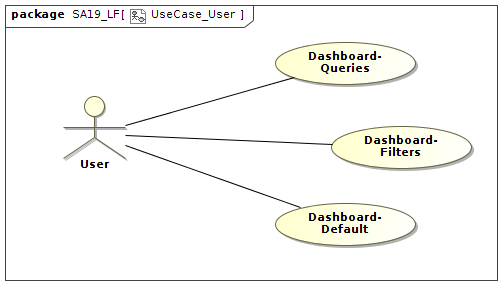
\includegraphics[width=\textwidth]{img/UseCase_User.png}
\caption{Use case diagram of the actor \textbf{User}.}
\end{figure}

\subsubsection{Tool use case diagram}
\begin{figure}[H]
\centering
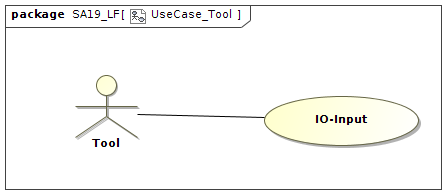
\includegraphics[width=\textwidth]{img/UseCase_Tool.png}
\caption{Use case diagram of the actor \textbf{Tool}.}
\end{figure}

\subsubsection{System use case diagram}
\begin{figure}[H]
\centering
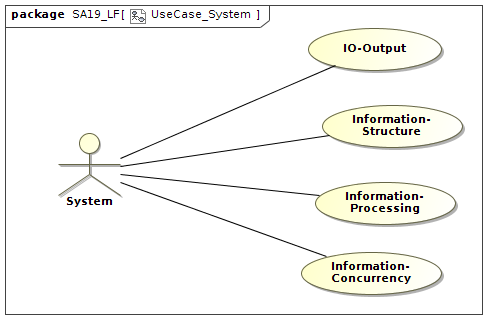
\includegraphics[width=\textwidth]{img/UseCase_System.png}
\caption{Use case diagram of the actor \textbf{System}.}
\end{figure}

\subsection{Tabular description of the most important requirements}
\begin{table}[H]
\caption{Information-Processing table}
\begin{tabular}{ |c|c| }
				\hline
 				\textbf{Use case name} & Information-Processing  \\
 				\hline
 				\textbf{Participating actors} & Tools, External system, system  \\
 				\hline
  				\textbf{Description} & 
      				\begin{tabular}{c}
      				     After that the system has collected \\
      				     the information sent by a tool,\\
      				    it processes it adding data, \\
      				    and stores it into the database system
      				\end{tabular} \\ 
 				\hline
 				\textbf{Triggering event} & Information receiving \\ 
 				\hline
 				\textbf{Priority} & High, level 5 \\ 
 				\hline
\end{tabular}
\end{table}
\begin{table}[H]
\caption{IO-Input table}
\begin{tabular}{ |c|c| } 
				 \hline
 				\textbf{Use case name} & IO-Input  \\
 				\hline
 				\textbf{Participating actors} & Tools, system  \\
 				\hline
  				\textbf{Description} & 
      				\begin{tabular}{c}
      				     Whenever a tool sends information, \\
      				     the system has to capture it in any case\\
      				\end{tabular}\\ 
 				\hline
 				\textbf{Triggering event} & Information receiving \\ 
 				\hline
 				\textbf{Priority} & High, level 5 \\ 
 				\hline
\end{tabular}
\end{table}
\begin{table}[H]
\caption{Dashboard-Default table}
\begin{tabular}{ |c|c| } 
				 \hline
 				\textbf{Use case name} & Dashboard-Default  \\
 				\hline
 				\textbf{Participating actors} & User, system  \\
 				\hline
  				\textbf{Description} &
      				\begin{tabular}{c}
      				     	Whenever the user execute the dashboard, \\
          				    the system should prints a default query
          			\end{tabular}\\ 
 				\hline
 				\textbf{Triggering event} & Dashboard request \\ 
 				\hline
 				\textbf{Priority} & Medium-High, level 4 \\ 
 				\hline
\end{tabular}
\end{table}

\section{Informal Description of the System \& its Software Architecture}

\subsection{Description of the System}

The system is composed of different high level components:
\begin{itemize}
    \item \textbf{fab\textunderscore data connector}: Under the assumptions described in the section \ref{first_design_decision}, we get the events from the database fab\textunderscore data. So the purpose of this component is to constantly query the external database in order to insert these information into our system. The method used to stream from the fab\textunderscore data database is described in \ref{kafka_connect}.
    
    \item \textbf{raw\textunderscore data connector}: The purpose of this component is to query external raw\textunderscore data database in order to retrieve the 10Mb files that contain the recipe regarding a specific tool. The method used to stream from the raw\textunderscore data database is described in \ref{kafka_connect}.
    
    \item \textbf{Message Broker}: This is the main component of our system: it takes the information from  both the \textbf{fab\textunderscore data connector} component and the \textbf{raw\textunderscore data connector}, manipulates them and performs message translation \& processing.  After the computation, this component stores its results in the \textit{analytics\textunderscore database}\\
    It also manages the information that the final users can monitor in the dashboard after applying the selected filters, The result information are retrieved from the \textit{analytics database}.
    
    \item \textbf{Analytics Database}: This the component responsible for the storage of the information. It contains the database itself but also DBMS and a controller used to perform storage operations (insertion,selection, etc). When the user apply specific filters in the dashboard these information has to be retrieved in this component's database.
\end{itemize}

\subsection{Architectural Pattern}
The team has decided to use \textbf{Publish/Subscribe} pattern, major information are in \ref{second_design_decision}.

\subsection{System boundaries}
External Components:
\begin{itemize}
    \item The database raw\textunderscore data is provided by the customer and so are the information regarding the recipes. The database is assumed to be reliable and fault tolerant. Also the information stored in it are assumed to be consistent and updated in real time. This system will be simulated in our prototype but without their non-functional requirements.
    \item The database fab\textunderscore data is provided by the customer and so are the information regarding the tools event. The database is assumed to be reliable and fault tolerant. Also the information stored in it are assumed to be consistent and updated in real time. This system will be simulated in our system prototype but without their non-functional requirements.
    \item A \textbf{network} with an architecture that is able to support the needed ratio of information. 
\end{itemize}

\subsection{Informal Diagram of the System}

\begin{figure}[H]
\centering
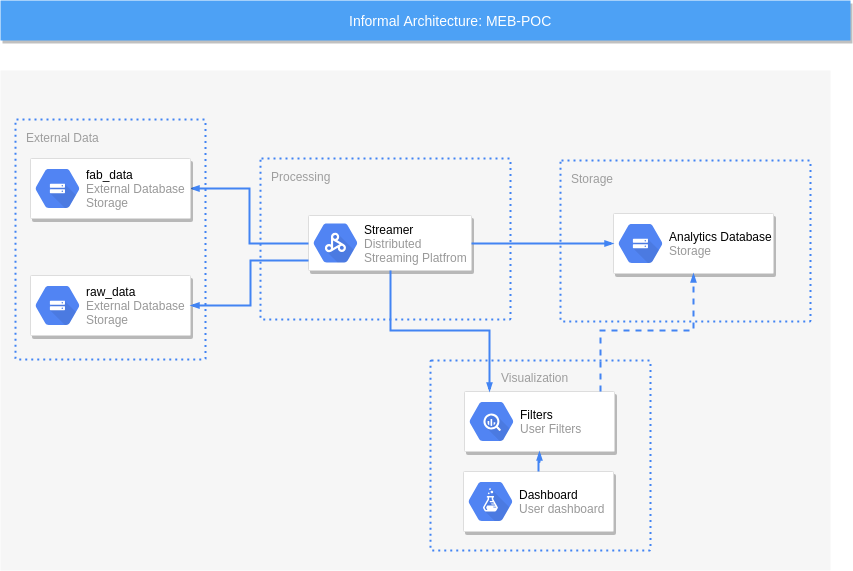
\includegraphics[width=\textwidth]{img/InformalDiagram.png}
\caption{Informal architecture of the system.}
\end{figure}

\subsection{Requirements' Fulfillment}
The requirements have been fulfilled in the following way:
\begin{itemize}
    \item \textbf{Dashboard-Queries}: The dashboard allows the user to perform queries on the data provided by the system's tools. There are two major REST endpoint, one \textit{/category/{n}} allows the user to get all the information regarding the category number {n}, the other \textit{/tool/{eqipID}} allows the user to get all the information about a specific tool identified by equipID. 
    \item \textbf{Dashboard-Filters}: The user has the possibility to apply filters.
    \item \textbf{Dashboard-Default}: The dashboard has an initial mode in which it will perform a default query.
    \item \textbf{Information-Structure}: The database system allows the storage of structured information about a specific tool into the Analytics database by using both a DBMS and the Kafka Embedded Database.
    \item \textbf{Information-Concurrency}: The database system allows concurrent operations like selection, update and insertion by using a JDBC specific driver.
    \item \textbf{Information-Processing}: The database system stores information about tools after they have been processed with additional predefined data provided by another system.
    \item \textbf{IO-Input}: The system is able to capture information from the tools in real time by using the interface to fab\_data and raw\_data databases which will publish the required information to their specific topics.
    \item \textbf{IO-Output}: The system provides the processed information in real time.
     \item \textbf{Scalability}: This is provided by the message broker.
    \item \textbf{Performance}:  The system is able to handle both the amount of requests and data as stated in the requirements.
    \item \textbf{Availability}: The developed system does respect this requirement.
    \item \textbf{Reliability}: The system architecture and the prototype are without Single Points of Failure. One tool that helps us in fulfilling this goal is the message broker that provides redundancy and fault tolerance.
\end{itemize}


\section{Design decisions}


\subsection{Tools' events (fab\_data capture) - fetching from DBMS vs sensor interception}
\label{first_design_decision}
  
    \begin{figure}[H]
\centering
 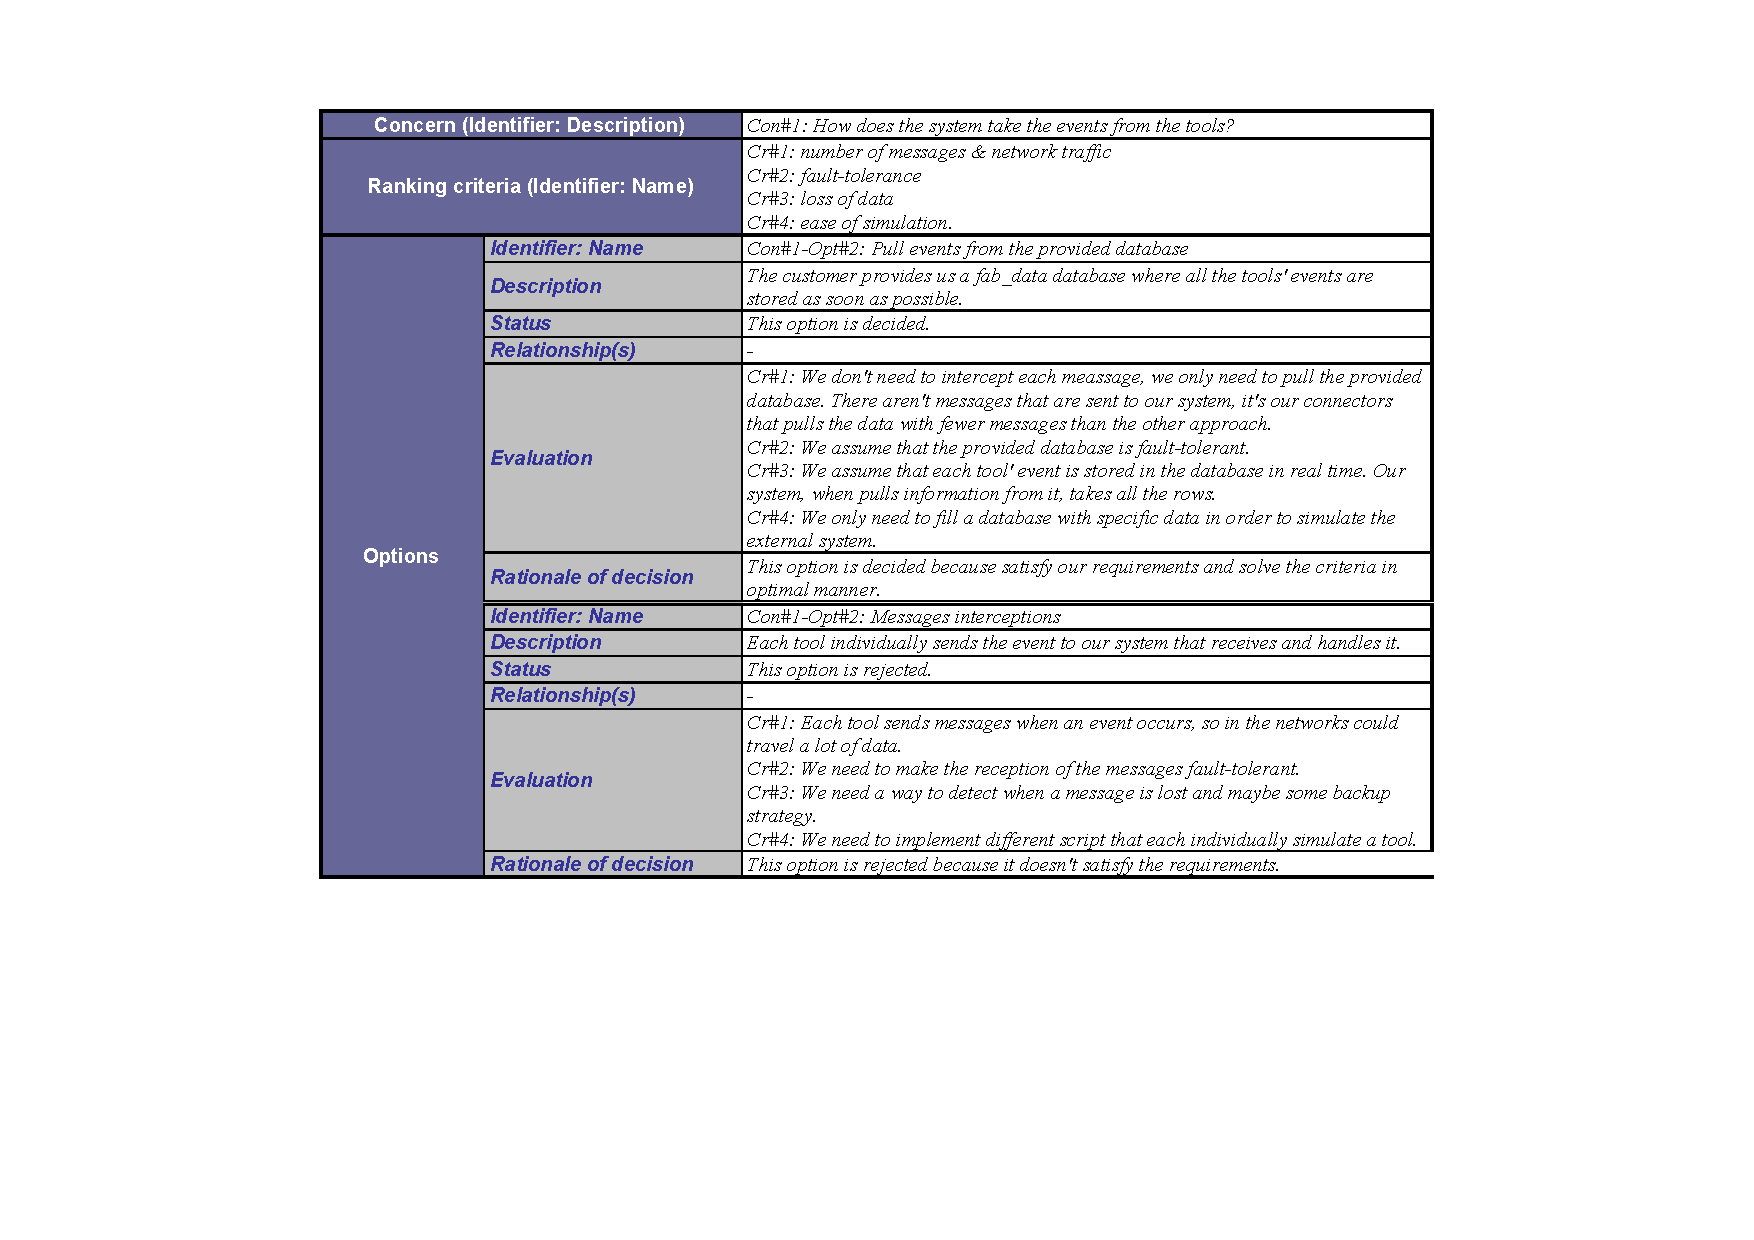
\includegraphics[trim=5cm 5.5cm 5cm 1cm,clip=true, width=\textwidth]{dd/dd1.pdf}
\caption{First design decision.}
\end{figure}
In order to prevent an high amount of messages towards our system which would be hard and time-consuming to manage individually, the team has decided to obtain the tools’ data from the \textit{fab\textunderscore data} database, which is provided externally.

The team assumes that the provided \textit{fab\textunderscore data} database is fault-tolerant and that the information are stored in it as soon as they are made available by their generating tools (in real-time).

This choice prevents loss of data in case of problems in the system’s connection, guarantees that every message will be retrieved by the system, makes it possible to eventually rebuild the history of messages.

\newpage
\subsection{Architectural Pattern}
\label{second_design_decision}
 \begin{figure}[H]
\centering
 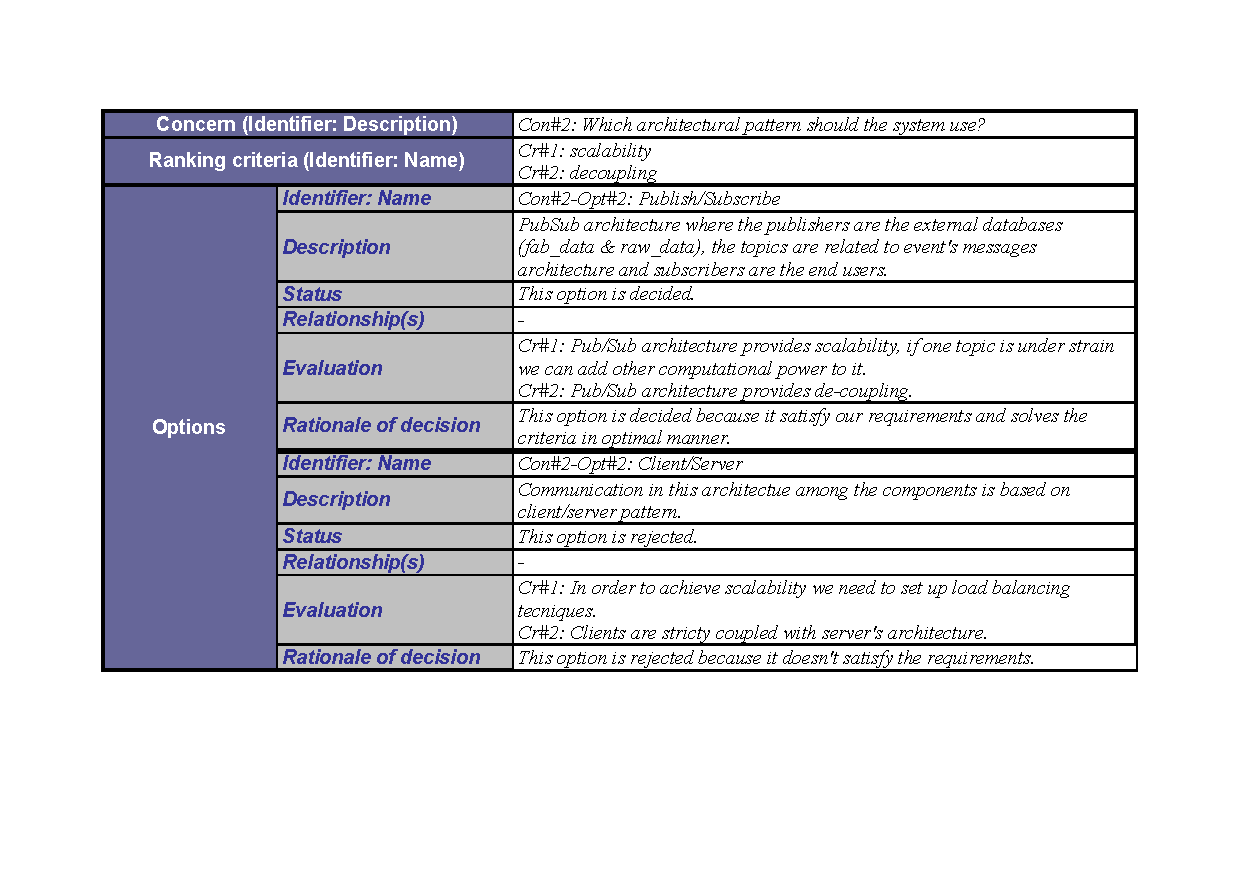
\includegraphics[trim=1.5cm 3cm 1.5cm 1.3cm,clip=true, width=\textwidth]{dd/dd2.pdf}
\caption{Second design decision.}
\end{figure}
The team has decided to opt for a Publish/Subscribe architecture. 
In the context of our application the publisher of the messages (i.e. the \textbf{producer}) is the component that gets the information from the \textit{fab\textunderscore data} database. So the messages of the system are the tools event (whose structure is described in the project specification). 
The \textbf{consumers} of the system are the users and the topics are the different categories. Components may subscribe to a set of events. It is the job of the publish-subscribe run-time infrastructure to make sure that each published event is delivered to all subscribers on that category.

We have decided to use this architectural pattern also because
Publish/Subscribe has great \textbf{scalability}, if we see that the current system is unable to satisfy our system constraints we can identify the most computationally loaded topics and subscribe other servers to these topics in order to parallelize their work (\textbf{horizontal scalability}). 
Another advantage is the \textbf{decoupling} of the system, publishers are loosely coupled to subscribers and so they are allowed to remain ignorant of system topology.


\subsection{From Message Broker to Streaming Platform}
\label{third_design_decision}

 \begin{figure}[H]
\centering
 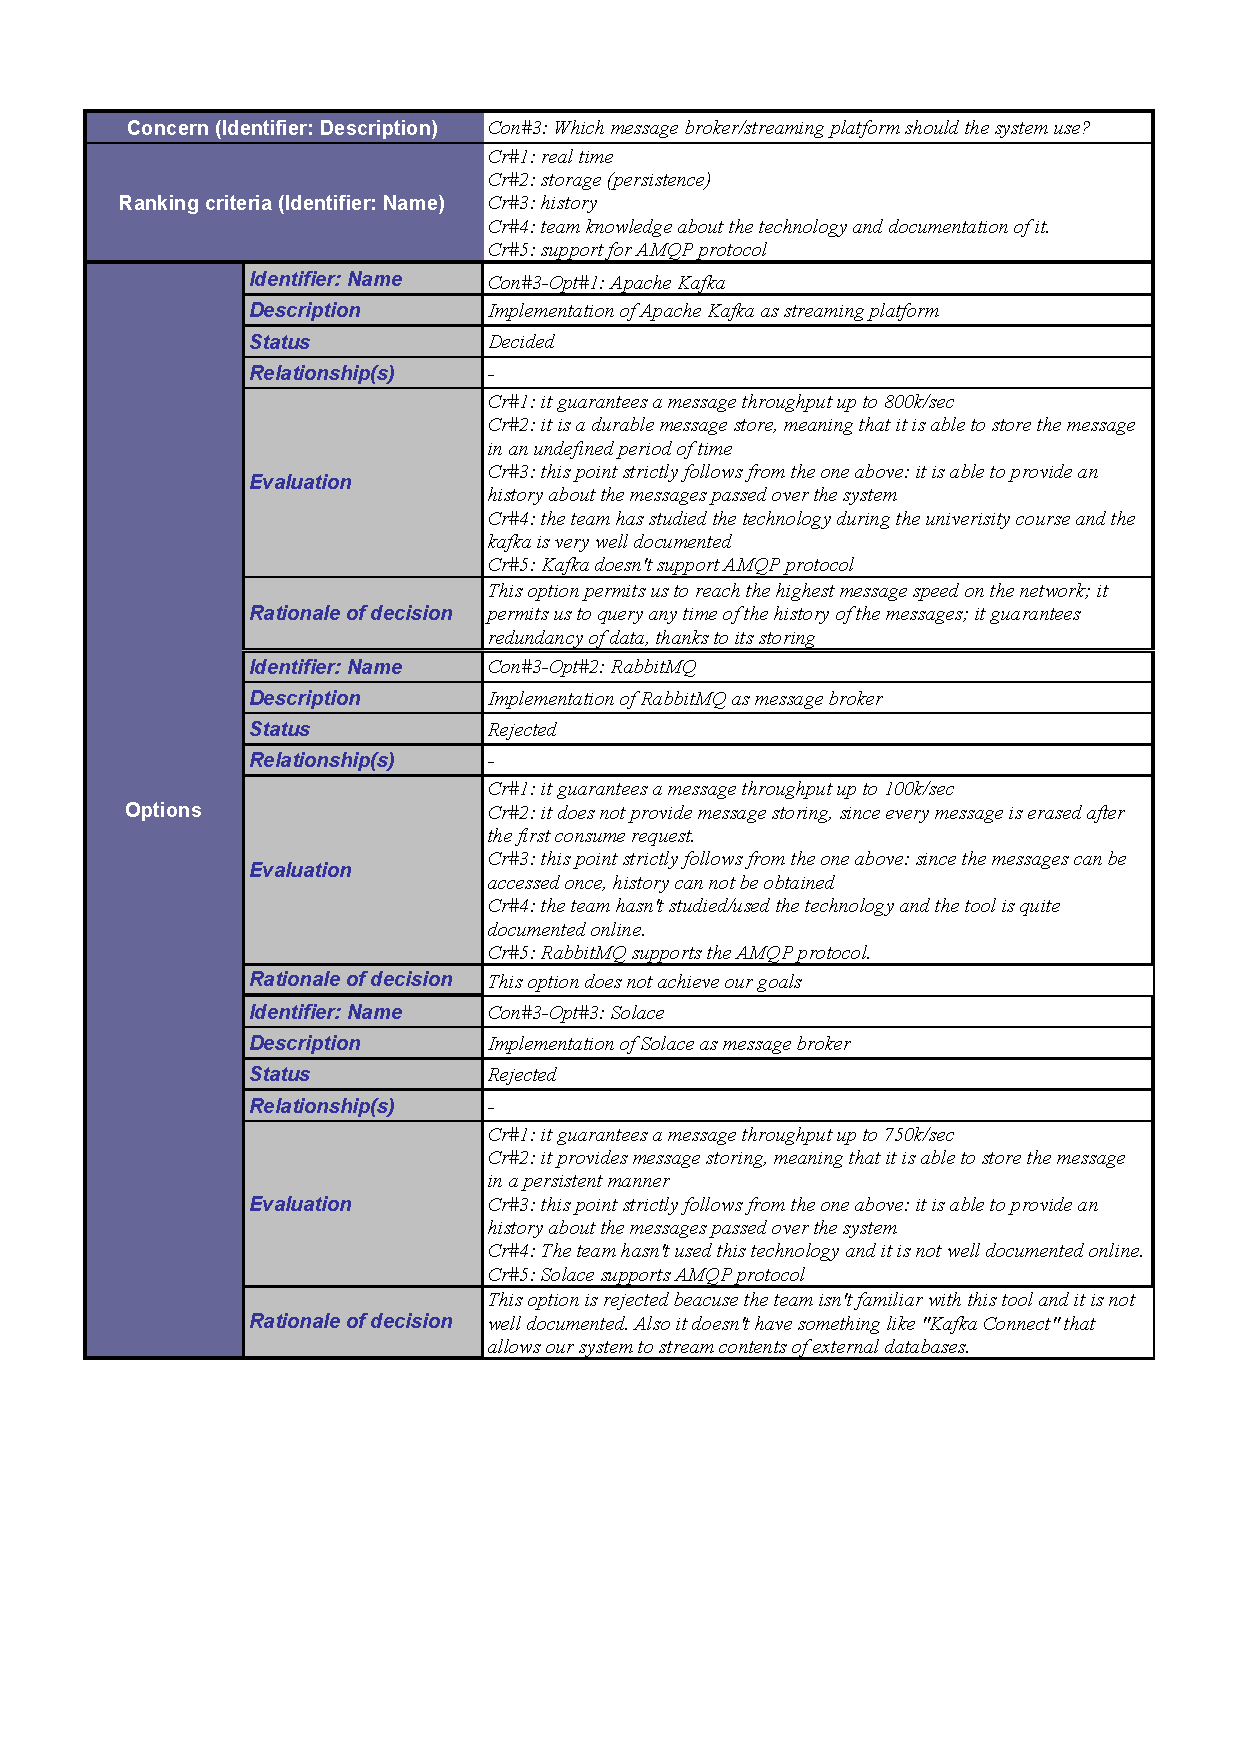
\includegraphics[trim=1cm 6.5cm 1cm 1.3cm,clip=true, width=\textwidth]{dd/dd3.pdf}
\caption{Third design decision.}
\end{figure}
\subsubsection{Apache Kafka}
In order to manage the messages, the team has decided to implement the Apache Kafka \textbf{Streaming Platform} instead of a conventional message broker.
Kafka perfectly complies with our needs\footnote{\url{https://content.pivotal.io/blog/understanding-when-to-use-rabbitmq-or-apache-kafka}}. It guarantees a very high throughput in terms of messages digested (peak of 800k/sec
\footnote{\url{https://engineering.linkedin.com/kafka/benchmarking-apache-kafka-2-million-writes-second-three-cheap-machines}}), which accomplishes our goal to afford the real time message processing. In this scenario, Kafka provides the fastest speed, compared to other message brokers like RabbitMQ, which could handle up to 100k/sec messages - due to its routing complexity.
Regarding storage, Kafka is better than RabbitMQ: Kafka is a durable message store, in which clients can get a \textit{replay} of the event stream on demand, as opposed to more traditional message brokers where once a message has been delivered, it is removed from the queue.
In our case this feature is useful since it permits to achieve a history of the messages which have passed through the system, and a recovery plan in case of malfunction, since Kafka permits the storage of the data.

\subsubsection{Kafka Connect}
\label{kafka_connect}
Another reason that favors Kafka over other Message Borker is Kafka Connect API\footnote{\url{https://docs.confluent.io/current/connect/index.html}}, more specifically a \textbf{Source Connector} which could "ingest entire databases and stream table updates to Kafka topics.". This is exactly the way in which the team has decides to pull information from the external \textit{fab\textunderscore data} and \textit{raw\textunderscore data} databases.

There are also two different ways that could be used in order to implement this external database "streaming" as states in this article\footnote{\url{https://www.confluent.io/blog/no-more-silos-how-to-integrate-your-databases-with-apache-kafka-and-cdc}}, either by using a JDBC plugin for the database's driver or by using \textbf{CDC} (i.e. \textit{Log-based Change-Data-Capture}). The team has opted for the CDC, in particular by using the Debezium\footnote{\url{https://debezium.io/}} platform.

\subsection{Recipes' Retrieval - raw\_data caching}
\label{forth_design_decision}
 \begin{figure}[H]
\centering
 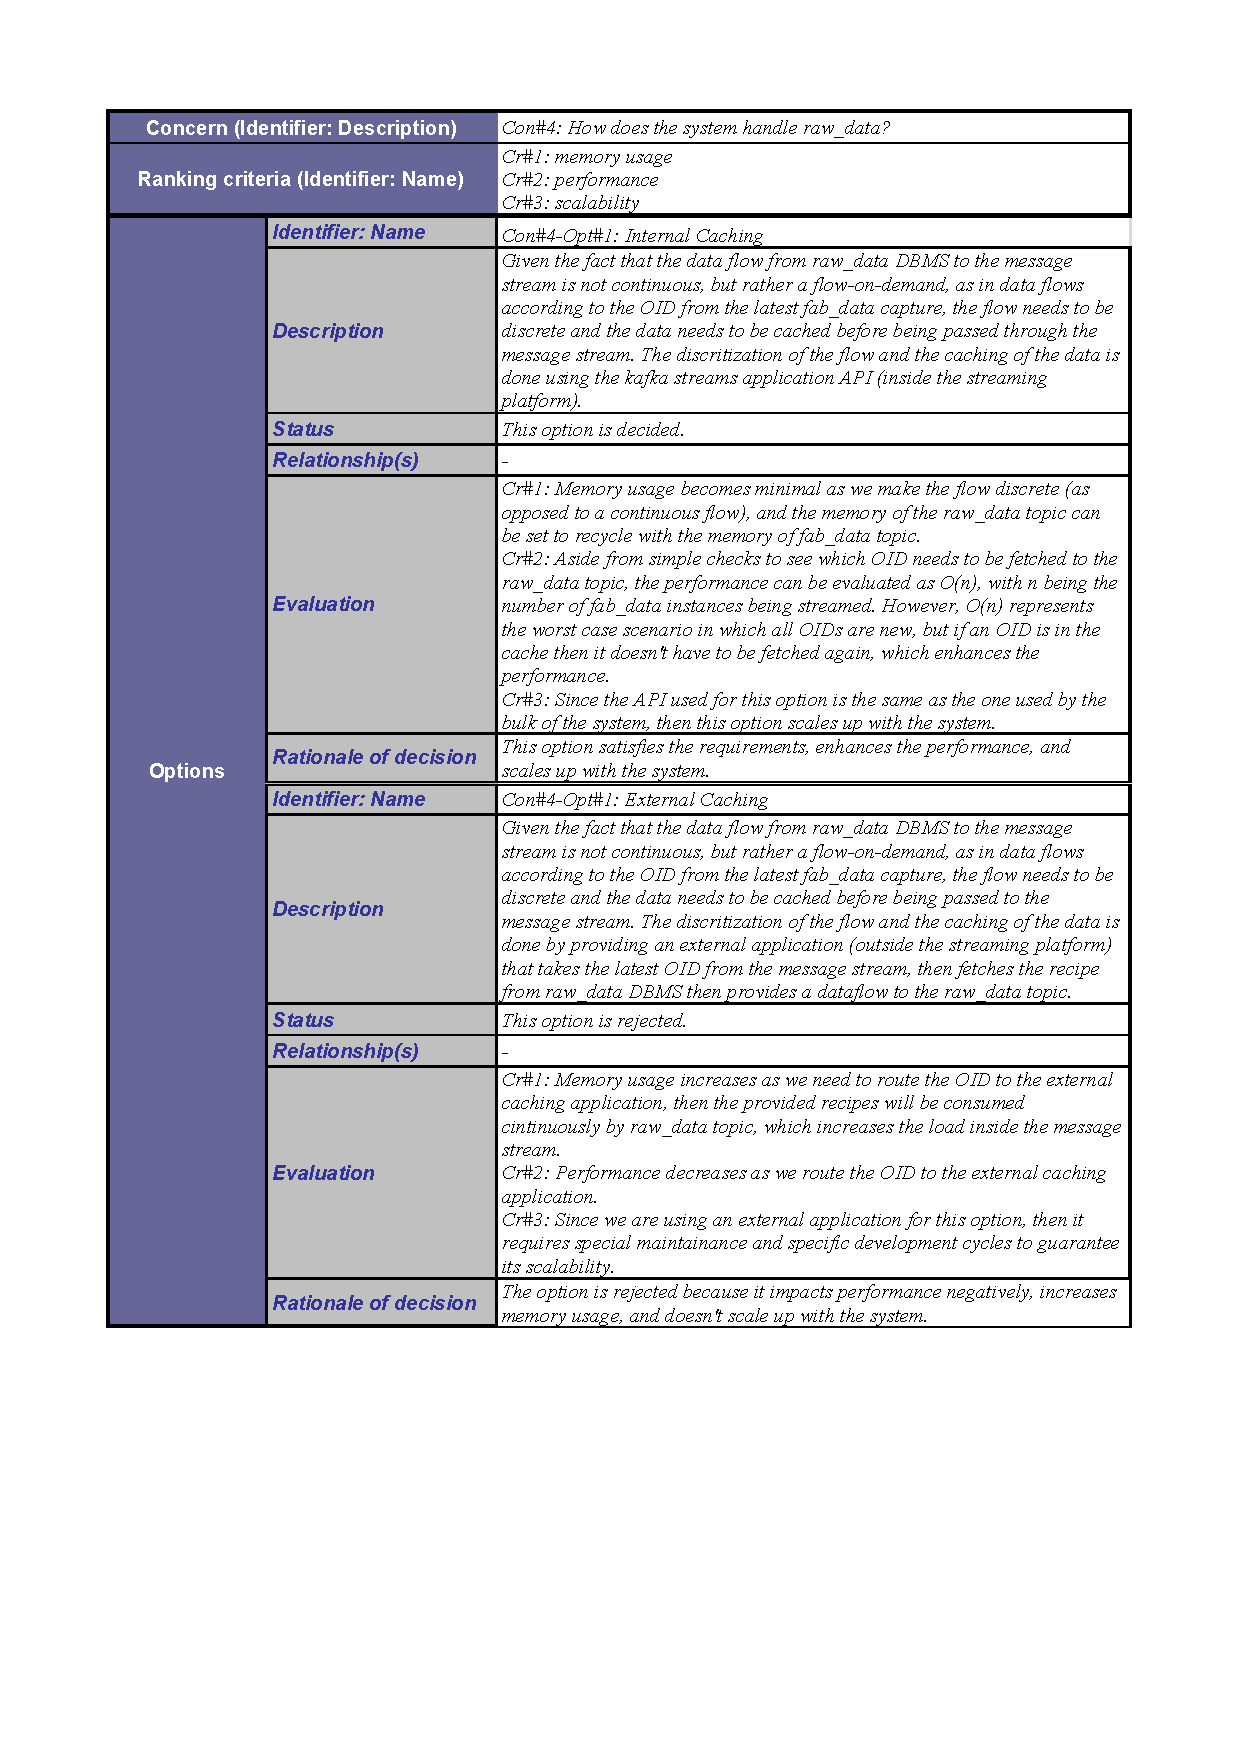
\includegraphics[trim=1.3cm 6.5cm 1.3cm 1.3cm,clip=true, width=\textwidth]{dd/dd4.pdf}
\caption{Forth design decision.}
\end{figure}

In order to integrate the process of recipe retrieval from the raw\_data DBMS, the team has decided to build an integrated discrete cashing methodology within the streaming platform using its own API.\\
This methodology allows for a dataflow-on-demand from the raw\_data DBMS only when needed, robust and interlocked development cycle, and scalability out of the box.

\subsection{Storage}
\label{firfth_design_decision}
 \begin{figure}[H]
\centering
 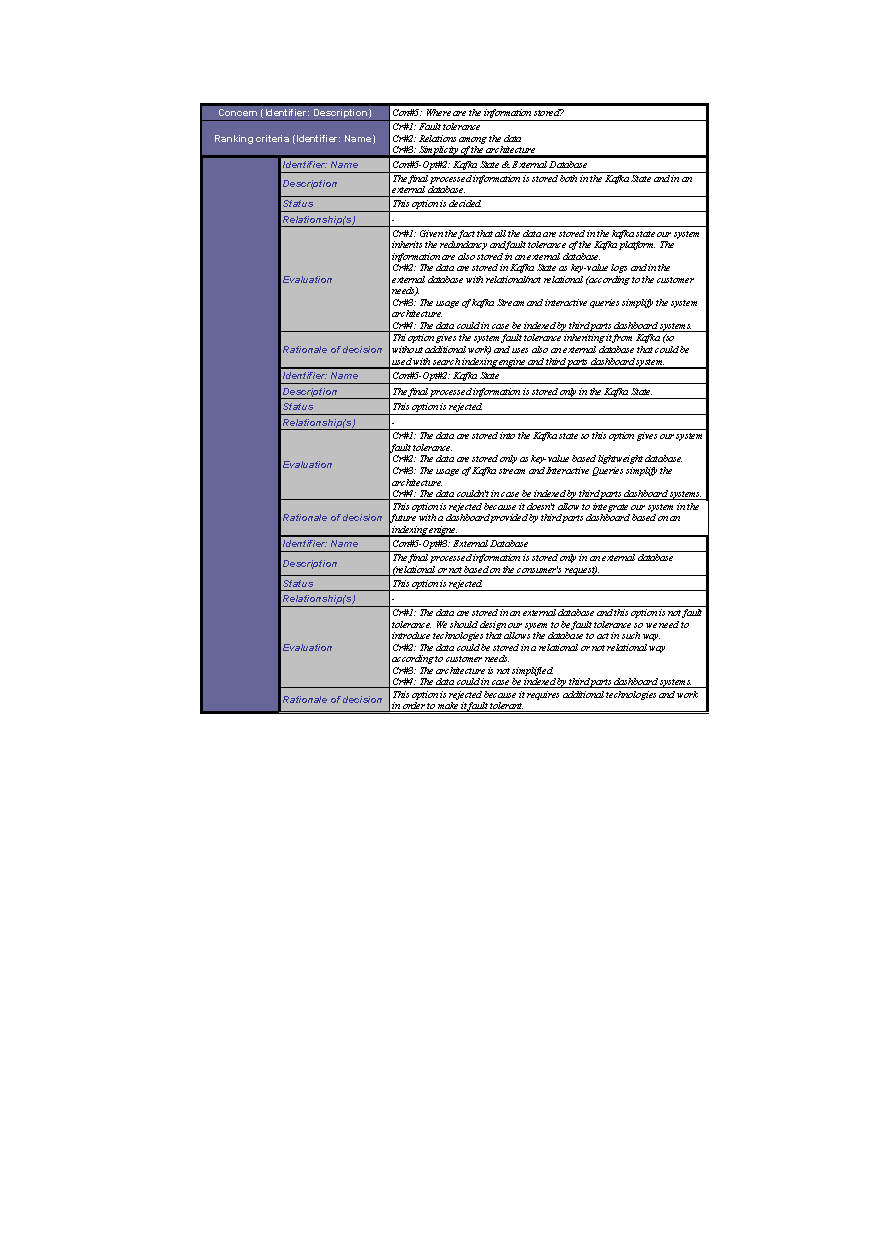
\includegraphics[trim=2.5cm 8.5cm 2.5cm 1.3cm,clip=true, width=\textwidth]{dd/dd5.pdf}
\caption{Fifth design decision.}
\end{figure}

In our system we need to store the  analytics information in a database.

In the project specification there are two constraints, our system needs to handle 80.000 messages every 30 minutes (Constraint 1) and should be able to scale up to 160.000 messages every 30 minutes (Constraint 2). So the messages flow is the following:

\begin{table}[H]
\caption{Messages ratio table}
\centering
\begin{tabular}{ |c|c|c| } \hline
\multicolumn{2}{|c|}{\textbf{Number of messages}} & \multirow{2}{2em}{\textbf{Time}} \\ \cline{1-2}
\textbf{Constraint 1} & \textbf{Constraint 2} & \\ \hline
80.000 & 160.000 & 30 min \\ \hline
$\approx2.700$ & $\approx5.200$ & 60 sec \\ \hline
$\approx45$ & $\approx 90$ & 1 sec \\ \hline
\end{tabular}
\label{table1}
\end{table}

Also the user, by using dashboard, could request both real-time and past information.
In order to provide the user with the real-time information the team has decided that the user could subscribe to the requested topics (i.e. the topics where the translated information are published).
As for the queries of past information the team has decided to use Interactive Queries provided by Apache Kafka, which makes the interrogation on kafka's logs, so they use the streaming platform also as permanent storage. This approach is discussed in the official documentation \footnote{\url{https://docs.confluent.io/current/streams/concepts.html\#interactive-queries}}.
The team has decided to store the information also in an external database (which could be relational or not relational but in our prototype we used a MongoDB's one) because in this way we could extend our system with real-time and non-real-time dashboard provided by third parts software which require traditional databases (like Kibana). 


\section{Views and Viewpoints}
\textbf{Stakeholders:}
\begin{itemize}
    \item \textbf{Sensor Engineer}: Responsible for designing and implementing the sensor networks. 
    \item \textbf{Core Developer}: Designs the communication system and the streams application (built using the streaming platform) that process our data. 
    \item \textbf{Database Developer}: Designs and administrates the database where our information are stored.
    \item \textbf{UI Designer}: Responsible for developing the dashboard where the information will be displayed.
    \item \textbf{System Integrator}: Responsible for system integration, emergency response and system migration.
    \item \textbf{End Users}: The final user of our system.
\end{itemize}
\begin{colortable}{Concern-Stakeholder Traceability}
& \textbf{\footnotesize Sensor Engineer} & \textbf{\footnotesize Core Developer} & \textbf{\footnotesize Database Developer} & \textbf{\footnotesize UI Designer} &  \textbf{\footnotesize System Integrator} & \textbf{\footnotesize End User} \\ \hline
Security &  & X & X &  & X & \\ \hline
Cost & X & X & X & X & X & \\ \hline
\footnotesize Networking \& Communication & & X & & & X & \\ \hline
Data Analysis & X & X & & & & X \\ \hline
Response Time & & X & X & & X & X \\ \hline
\makecell{ Depend-\\ ability} & X & X & X & X & X & \\ \hline
Usability &  &  &  &  &  & X \\ \hline
\makecell{Scala-\\bility} & & X & & & X & \\ \hline
Energy Consumption & X & X & & & & \\ \hline
\end{colortable}
\chapter{Project Architecture}
\section{Component Diagram}
\pagebreak
 \begin{figure}[H]
\centering
 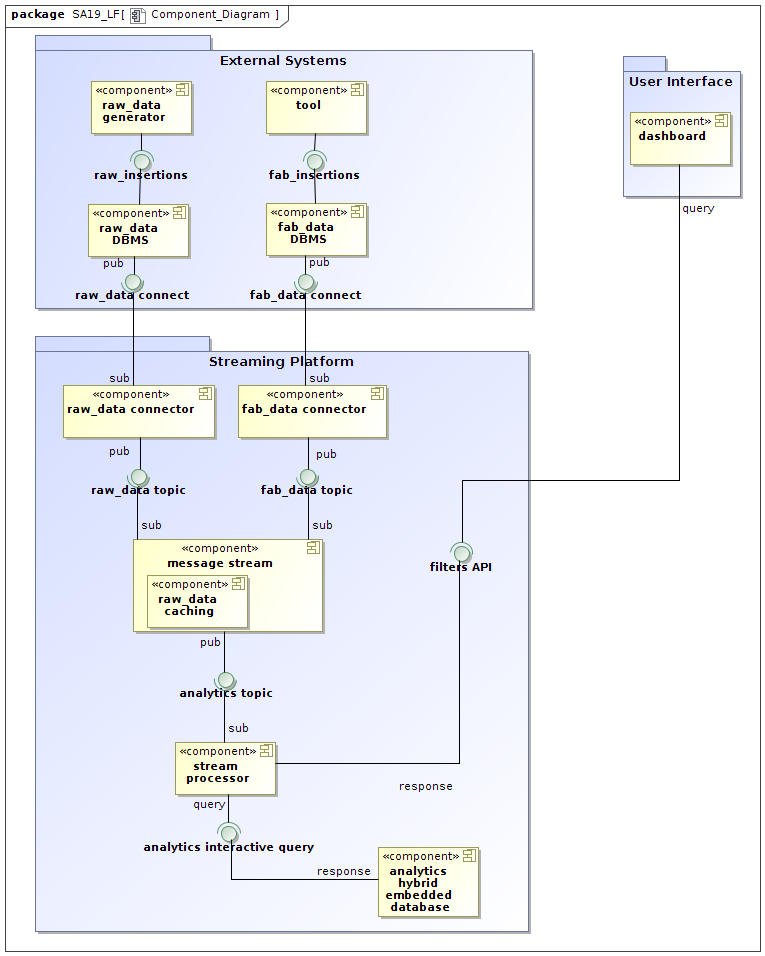
\includegraphics[width=\textwidth, height=\textheight]{img/Component_Diagram.png}
\caption{Component diagram.}
\end{figure}

\subsection{Components Description}
\begin{itemize}
    \item External Systems Package: This package contains the external databases and systems which our system depends upon.
    This package represents everything that is provided by the customer.
    \begin{itemize}
        \item \textbf{raw\_data DBMS}: This component refers to the external database raw\textunderscore data.
        \item \textbf{fab\_data DBMS}: This component refers to the external database fab\textunderscore data.
        \item \textbf{raw\_data generator}: This component refers to an external system that inserts data into the external database raw\_data.
        \item \textbf{tool}: This component refers to the external tool that generates events and inserts them into the fab\textunderscore data database.
    \end{itemize}
    \item Streaming Platform Package:
    \begin{itemize}
        \item \textbf{fab\textunderscore data connector}: This component is responsible for streaming the event messages (received by the external fab\textunderscore data database via a specific tool interface) into a Kafka topic called fab\_data topic.
        \item \textbf{raw\textunderscore data connector}: This component is responsible for streaming the translation messages (received by the external raw\textunderscore data database via a specific tool interface) into a Kafka topic called raw\_data topic.
        \item \textbf{message stream}: This component is subscribed to two topics: fab\_data topic \& raw\_data topic. It is responsible for the translation of the fab\_data events. In order to do this, this component uses internal caching.
        \item \textbf{raw\_data caching}: This component is used to cache the information taken from the raw\_data database by using raw\_data topic. It caches  the latest pair (OID, nameTranslation) received for each id (which could be eqipOID, recipeOID, stepOID). Therefore it allows for a raw\_data:fab\_data relationship in the system of 1:n.
        \item \textbf{stream processor}: This component does the following:
        \begin{itemize}
            \item consumes translated information from the specific topics and stores them into the analytics DBMS, both the Kafka one and the MongoDB one.
            \item applies both default and user-specified filters to the analytics information.
            \item sends requests to the analytics DBMS according to some of the filters (for getting past information).
            \item provides the analytics information (past and current) to the dashboard.
        \end{itemize}
        \item \textbf{analytics hybrid embedded database}: This component is responsible for the storage of the tools' information.
    \end{itemize}
    \item User Interface Package:
    \begin{itemize}
        \item \textbf{dashboard}: This component is responsible for the visualization of the stored information. Also it allows the final user to apply specific filters on the requested data. 
    \end{itemize}

\end{itemize}

\subsection{Interfaces Description}
\begin{itemize}
    \item External Database Package:
    \begin{itemize}
        \item \textbf{raw insertions}: This interface represent the communication between the raw\_data generator and the raw\_data DBMS. 
        \item \textbf{fab insertions}: This interface represent the tool(s) and fab\_data DBMS. 
        \item \textbf{raw\_data connect}: This interface is responsible for the communication between the external database raw\textunderscore data and our system. This communication is discrete, and happens on demand by our system.
        \item \textbf{fab\_data connect}: This interface is responsible for the communication between the external database fab\textunderscore data and our system. This communication has to be in real-time, as soon as a new entry is inserted into the database this interface has to provide it to our system.
    \end{itemize}
    \item Streaming Platform Package:
    \begin{itemize}
        \item \textbf{fab\_data topic}: This interface refers to all the topics that are used by the component fab\textunderscore data connector to stream the external fab\textunderscore data database.
        \item \textbf{raw\_data topic}: This interface refers to all the topics that are used by the component raw\textunderscore data connector to stream the external raw\textunderscore data database.
        \item \textbf{analytics topic}: This interface refers to all the topics in which the translated information are written so that the component \textit{message stream} can store them.
         \item \textbf{analytics interactive queries}: This interface performs CRUD operations with the analytics DBMS.
    \end{itemize}
    \item Analytics Package:
    \begin{itemize}
        \item \textbf{filters API}: This interface is responsible for the communication between the user's dashboard and our system.
    \end{itemize}
\end{itemize}

\section{Sequence Diagram}

\subsection{Dashboard}

This diagram represents the actions' flow of a query made by an end user on the dashboard. This component will send a message to the stream processor component, which is responsible of the analytics message flow. If the time concerning the query is the present, it means that the end user is interested in some part of the flow which is passing through the stream processor at the current moment, and the processor will consume the interested data; otherwise, it will send a MakeQuery() message to the hybrid embedded analytics database, located in our system. In this database all the analytics data are stored, and it's where the system will search to answer queries about past information.
In both cases, the dashboard will receive a return.


\begin{figure}[H]
\centering
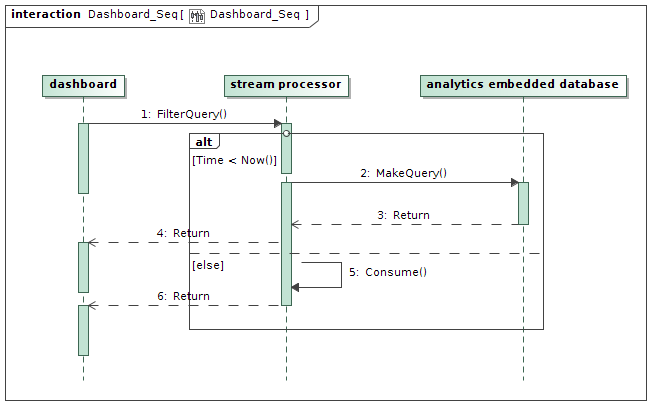
\includegraphics[width=\textwidth]{img/Dashboard_Seq.png}
\caption{Sequence diagram from the \textbf{dashboard} point of view.}
\end{figure}

\subsection{Raw\_data}
This diagram represents the events that occur when the raw\_data generator inserts new data into the database. Of course, this means that it will send an Insert message to the raw\_data DBMS, which in turn will publish this value on its Kafka topic, namely the raw\_data connect, at which the raw\_data connector is subscribed and in turn will send a consume operation. After that the raw\_data connector will publish the processed message in the raw\_data topic.

\begin{figure}[H]
\centering
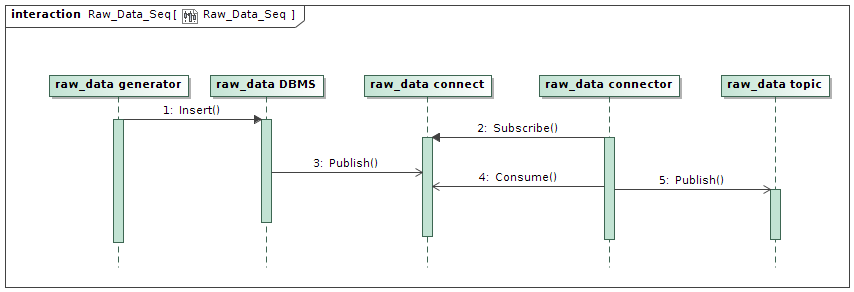
\includegraphics[width=\textwidth]{img/Raw_Data_Seq.png}
\caption{Sequence diagram from the \textbf{raw\_data} point of view.}
\end{figure}

\subsection{Fab\_data}

\begin{figure}[H]
\centering
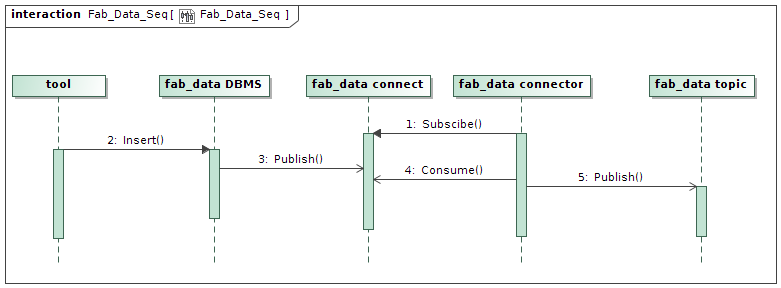
\includegraphics[width=\textwidth]{img/Fab_Data_Seq.png}
\caption{Sequence diagram from the \textbf{fab\_data} point of view.}
\end{figure}

This diagram represents the events that occur when a tool inserts an event into the external database. When this happens the fab\_data connector (which was subscribed to that topic) receives the new event and, after some computation, publishes it in the new fab\_data topics.

\subsection{Streaming}
\begin{figure}[H]
\centering
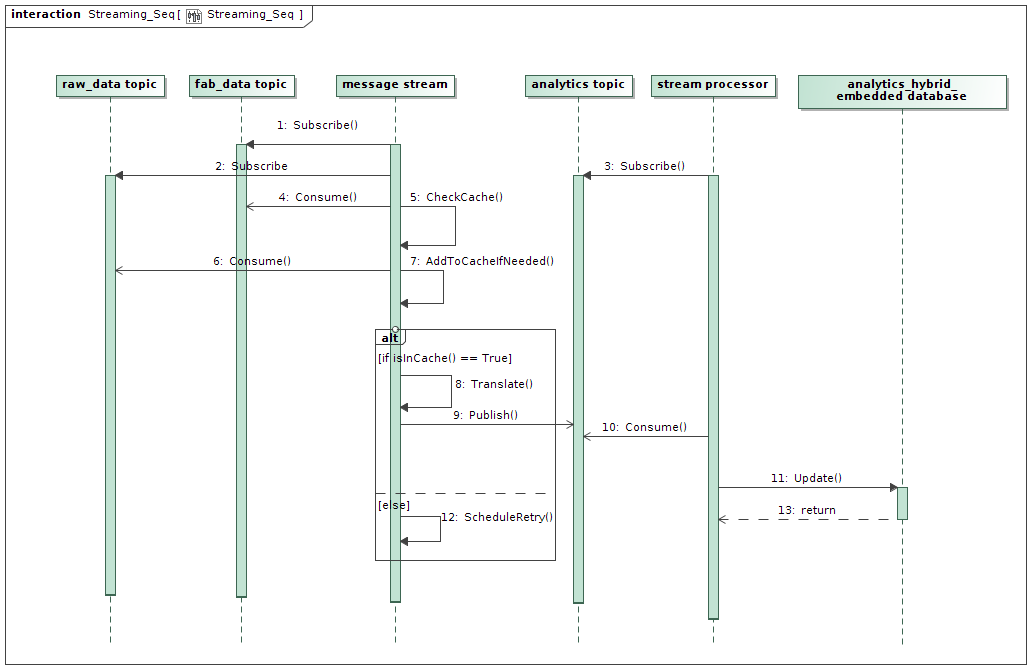
\includegraphics[width=\textwidth]{img/Streaming_Seq.png}
\caption{Sequence diagram of the \textbf{Streaming platform} flow of events.}
\end{figure}

This diagram represent the actions taken by the streaming platfrom package. the \textit{Message Stream} subscribes to both fab\_data and raw\_data topics then when there is a publication of a new message on the fab\_data topic, the message is consumed by the message stream. Then the message stream compares the OID in the message to its cache, if a recipe with that OID is not present, it stores this failed translation into a specific kafka topic and it delays the translation so that it can retry later (every 30 sec). Else if the information are present, this component performs the translation and republishes the result into a specific output topics in the analytics\_topics interface. This message is consumed my the stream processor that stores it both in the kafka DB and, by using kafka connect, also in the external database.
\chapter{Second deliverable}
\section{CAPS}
\subsection{CAPS Diagrams}
\begin{figure}[H]
\centering
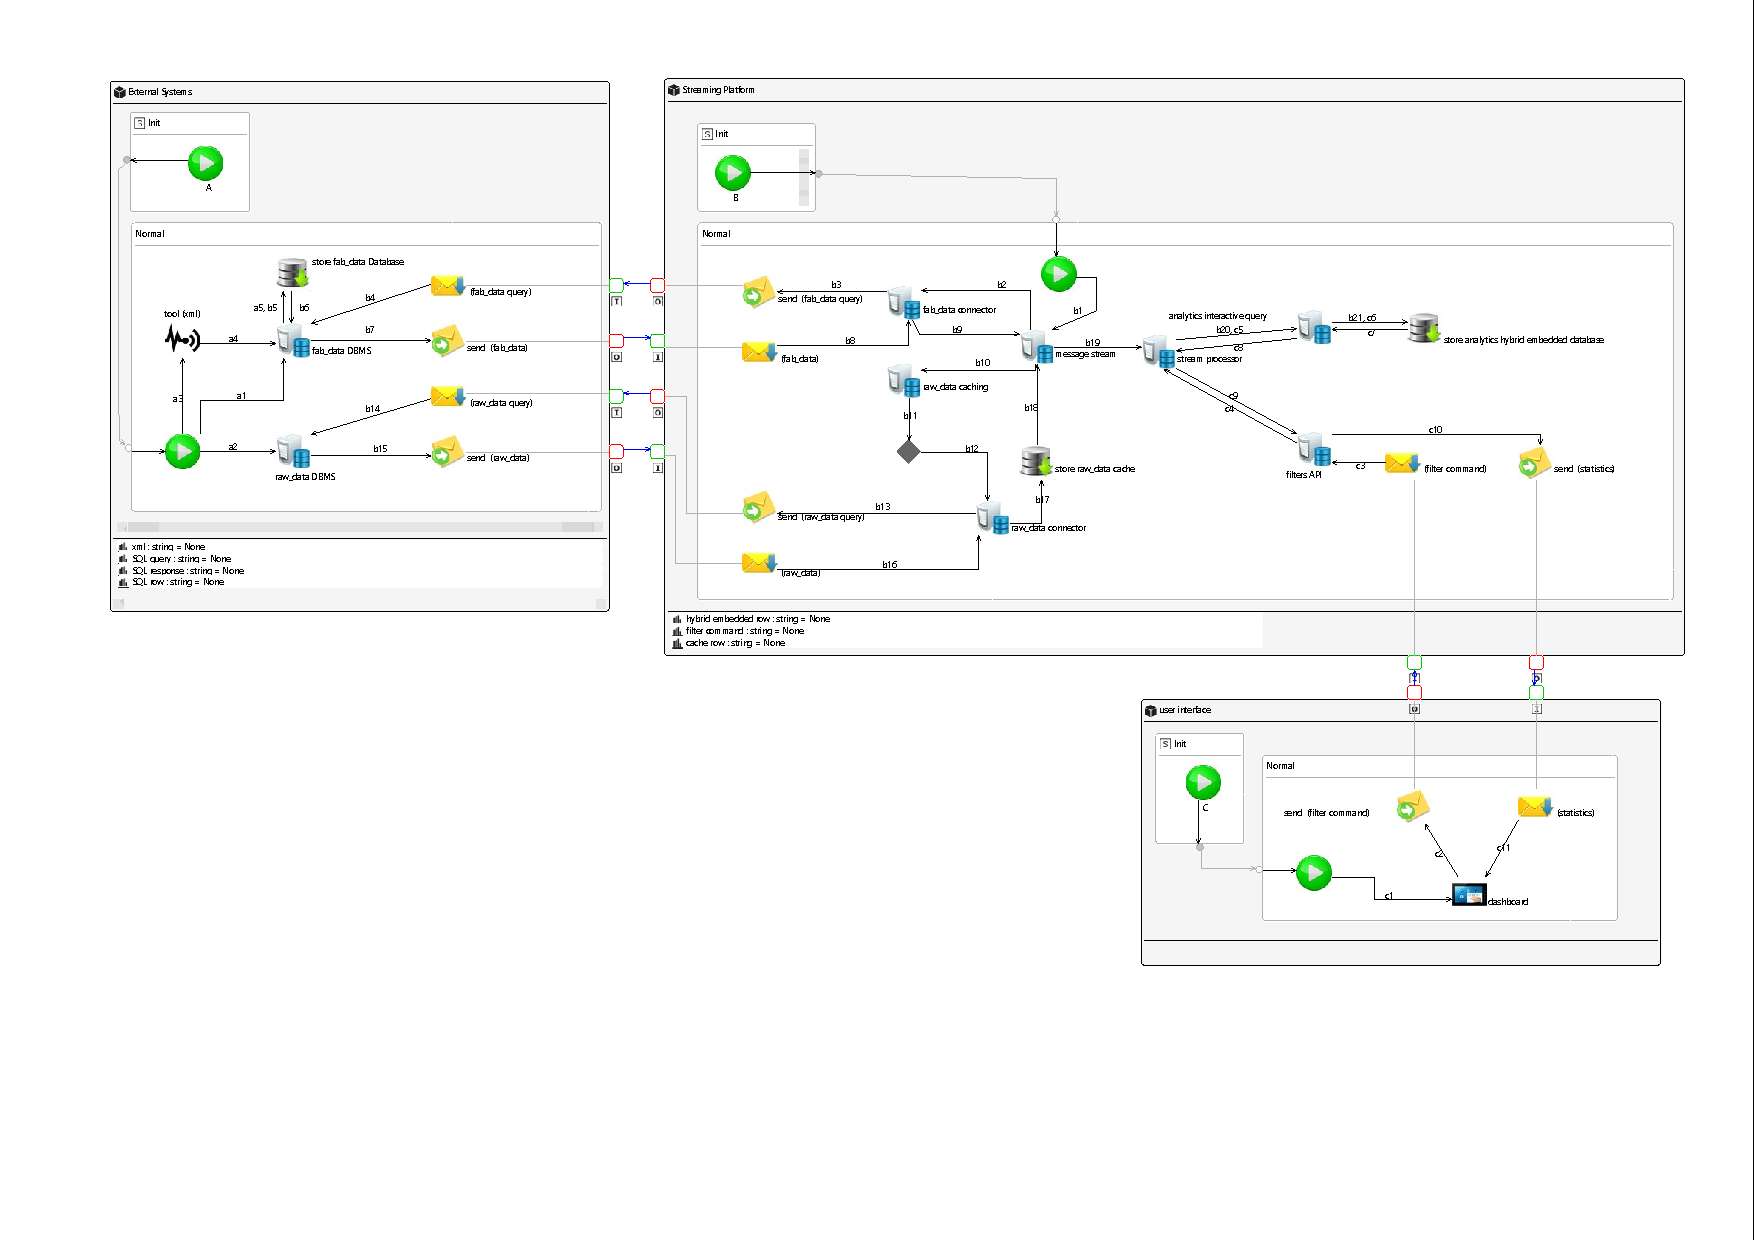
\includegraphics[trim={1.8cm 4cm 1cm 1.2cm},clip, width=\textwidth]{img/SAML.pdf}
\caption{SAML Diagram}
\end{figure}
The MEB-POC SAML Diagram source-code is downloadable from \href{https://drive.google.com/file/d/1ef9sZ7FFk_6fUsoZxO2Dyb8F9S59mnfx/view?usp=sharing}{Google Drive} and also available at \href{https://github.com/LuigiCerone/MEB-POC/tree/CAPS}{the "CAPS" branch of the project\'s github repository} (at the moment the repository is private).
\newpage
\subsection{CAPS Design Decisions}
\subsubsection{Design Decision 1}


\begin{figure}[H]
\centering
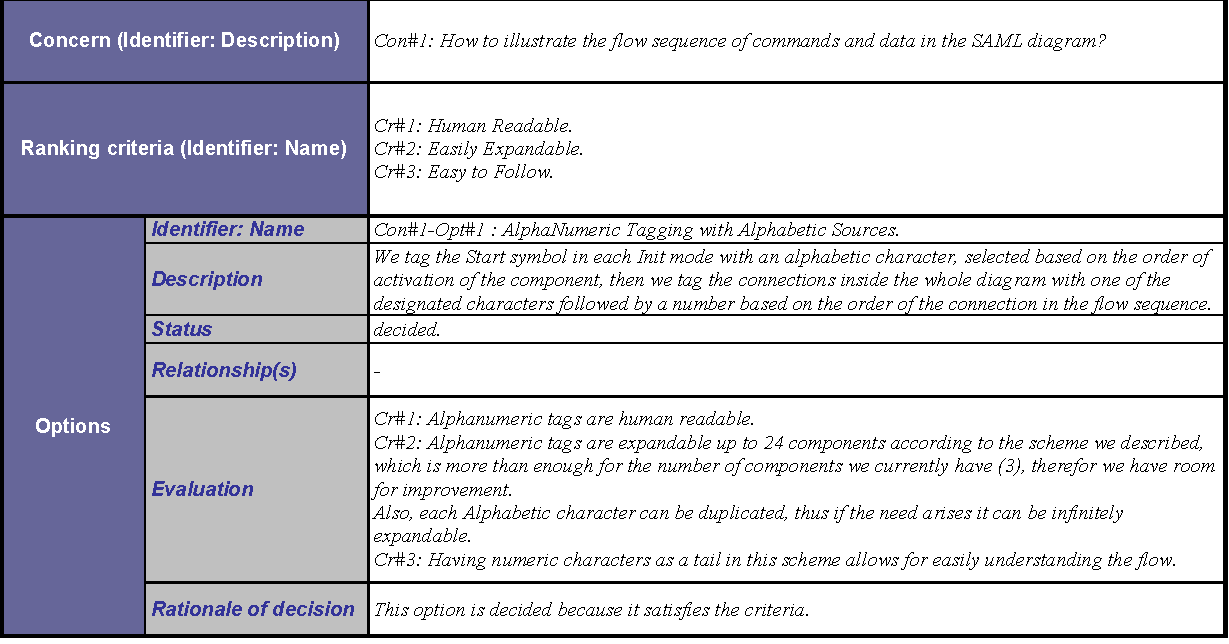
\includegraphics[width=\textwidth]{dd/DD-CAPS}
\caption{CAPS design decision}
\end{figure}

\subsubsection{Design Decision 2}
In the SAML diagram, we have decided to illustrate the tool output as XML, as indicated in the System Specification, it is therefore assumed that the fab\_data DBMS has a plugin or an extention capable of understanding that format and performing any necessary conversion of XML into a suitable format for the fab\_data database.
\newpage
\section{From architecture to code}

\subsection{Implemented service}
The system proposed in the previous chapters has been implemented in all its parts by using Kafka framework and by simulating the external databases with an ad-hoc tool developed by the team. The code for the MEB-POC system is downloadable from \href{https://drive.google.com/file/d/1CoNjQ_QpPEka4pH3k3aG3dxaqVhfUVZK/view?usp=sharing}{Google Drive} and is also available in \href{https://github.com/LuigiCerone/MEB-POC}{the "master" branch of the project\'s github repository} (at the moment the repository is private). The simulator's code is downloadable from \href{https://drive.google.com/file/d/1Qs3vJLEiLnZ-XM0G12GDj06ffdyb5ONJ/view?usp=sharing}{Google Drive} and, as above, available at \href{https://github.com/LuigiCerone/DBs\_Simulator}{github}(now the repository is private).
The language used is Java and there is an appendix chapter that tries to describe the steps needed to run the system on another laptop. \\
A short video that show the execution of the prototype is available at \\ \href{https://youtu.be/ARS0Be7CP28}{https://youtu.be/ARS0Be7CP28}. \\ 

Overall all the external dependencies of the system and the tools used by the team to develop it are:
\begin{itemize}
    \item Kafka Stream and Kafka Processor API,
    \item Jackson library for POJO serialization/deserialization,
    \item Jersey library for the RESTful interface used to implement the dashboard,
    \item MongoDB driver used to access an external backup database,
    \item Maven as dependencies manager,
    \item Git as version control manager.
\end{itemize}

The final translated information are stored both in the Kafka Stream Local State in a persistent way and also in an external MongoDB database.
The following is a diagram that represents the topics used in the system and that tries to explain the flow of information:

\begin{figure}[H]
\centering
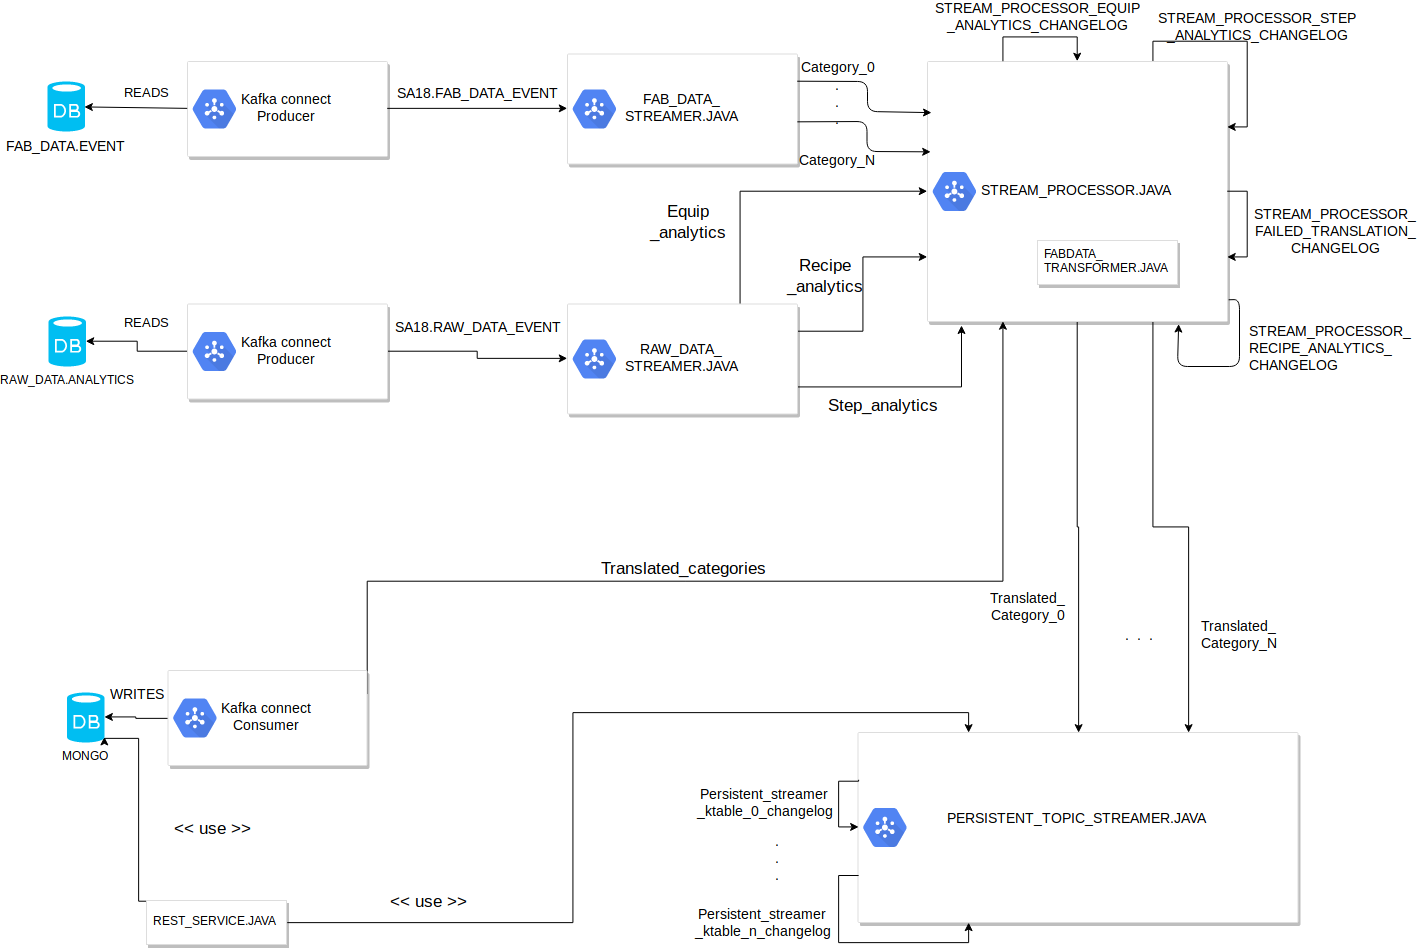
\includegraphics[width=\textwidth]{img/diagram_topics.png} \\
\caption{Used topics for the communcation}
\end{figure}


The text written above the lines represents the topic used to communicate between the classes. The topics: streamer-processor-equip\_analytics-changelog, streamer-processor-recipe\_analytics-changelog, streamer-processor-step\_analytics-changelog are \textbf{persistent} topics i.e. when the system is shut down the data they contains is not lost because it is written into the disk of the kafka's cluster computers. These topics contains the mappings used for translation in the form OID --> Translation. The topic streamer-processor-failed\_translations-changelog is another \textbf{persistent} topic where there are written the FabEvent that our system couldn't translate (major details about the translation topic is in the following section).
All the topics of the form persistent-streamer-ktable\_NUMBER-changelog are used to store the result of the translation for each category in a \textbf{permanent} way, in this way this information benefits of kafka fault tolerance and replication. Also, by using the Interactive Query API \footnote{\url{https://kafka.apache.org/10/documentation/streams/developer-guide/interactive-queries.html}}, these data could be queried with an SQL-like syntax\footnote{\url{https://www.confluent.io/product/ksql/}}.

The prototype has been implemented in package whose names respect the component diagram's one. The following is the class diagram relative to the Message Stream component:

 \begin{figure}[H]
\centering
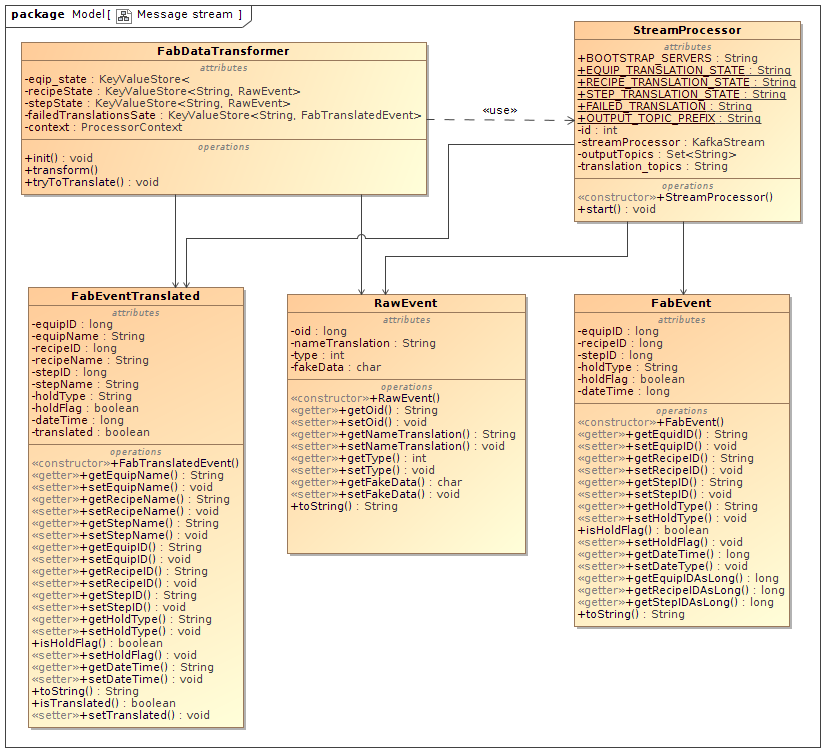
\includegraphics[width=\textwidth]{img/Class_Diagram.png} \\
\caption{Class diagram for package \textbf{message\_stream}}
\end{figure}

This package contains all the logic about the translation from a FabConnectEvent's object into a FabTranslatedEvent one. In the following section there is an activity diagram that describes the algorithm used to perform this operation.

\subsection{Translation logic}
\newpage

 \begin{figure}[H]
 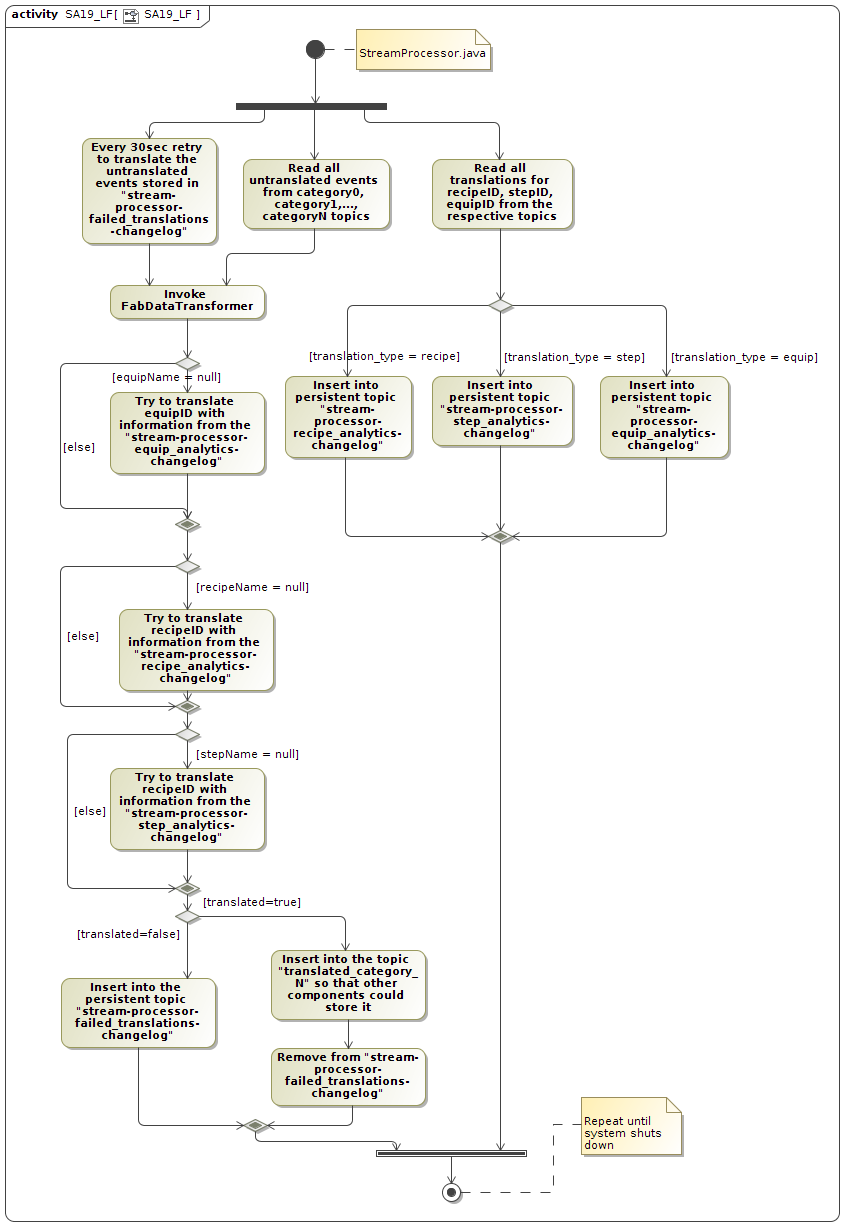
\includegraphics[width=\textwidth, scale=0.7]{img/activity.png}
\caption{Activity diagram for translation logic.}
\end{figure}

\subsection{Tests}
In the requirements section we said that our system should be albe to scale up to 160.000 msg every 30 mins. This means almost 5300 msg every minute, so one msg every 11ms.

\begin{table}[H]
\caption{Tests}
\centering
\begin{tabular}{ |c|c| } \hline
\textbf{Number of messages sent from simulator} & \textbf{Time} \\ \hline
6.600 & 75837ms $\approx 1 msg/11ms $ \\ \hline
\end{tabular}
\label{table1}
\end{table}
We did our tests on a single laptop, meaning that the pc was both running the simulator and the prototype of our system. So the kafka cluster was composed by only one pc. This means that in a production environment where there is a cluster of brokers among which the operations could be separated by using publish/subscribe architecture, our system could increase its performance. Also another thing to note about our tests is that the simulation of the external databases is computational expensive.

In order to test the size of the messages in the raw\_data database we added a fake field called fakeData used to grow the size of the message. We tried our system with it but, given the fact that the simulation requires high computational power, team thinks that the final stats could be further improved.


\section{Conclusion}

The system architecture proposed in the first chapter is based on a publish/subscribe pattern, implemented using the Kafka framework.
All the translated information are stored in the Kafka Streams local state and also in an external database (in our case a MongoDB's one).
The architecture (and so the prototype) has a series of advantages provided by the Kafka framework, such as:
\begin{itemize}
    \item If a producer loses the connection to the cluster it will wait for the connection to come back online without crashing or losing messages.
    \item If a consuming client loses the connection it will simply wait for the cluster to come back online and it will resume the consumption from where it left
    \item The information stored in the local state are replicated in the kafka cluster, in this way the final information are stored in a reliable and fault-tolerant manner.
    \item If there is a particular category in which the load of work is heavier with respect to the others, we can add more computational power to the kafka cluster thanks to its \textbf{horizontal scalability}.
    \item The components are decoupled from each other, this is a typical advantage of publish/subscribe architecture.
\end{itemize}

So, to summarize, we can say that the chosen architecture has proven us to be able to scale up to the requested messages ratio.
\begin{appendices}
\chapter{Installation notes}

Install mysql server and create an user with username \textit{sa18} and password \textit{software\_architectures\_18}. Grant to this user all the permission to perform CRUD operation.

In order to install kafka
\begin{lstlisting}[language=bash]
cd /home/USER_NAME/Downloads (or "Scaricati")
sudo wget http://it.apache.contactlab.it/kafka/2.1.0/kafka_2.11-2.1.0.tgz

tar xvzf kafka_2.11-2.1.0.tgz
mkdir /opt/kafka
sudo mv kafka_2.11-2.1.0/ /opt/kafka
 
\end{lstlisting}

In order to use Kafka Connect you need to install mysql on the computer and the configure the log of the DBMS. 
Edit the file \textit{/etc/mysql/my.cnf} by adding the line log\_bin = mysql-bin :

Example:
\begin{lstlisting}
[mysqld]
server-id         = 42
log_bin           = mysql-bin
binlog_format     = row
binlog_row_image  = full
expire_logs_days  = 10
\end{lstlisting}

and restart the mysql server.

Then we need to create two services, one for zookeeper and one for kafka.

\begin{lstlisting}[language=bash]
sudo nano /etc/systemd/system/zookeeper.service
\end{lstlisting}
 with code:
 \begin{lstlisting}
 [Unit]
Description=Apache Zookeeper server (Kafka)
Documentation=http://zookeeper.apache.org
Requires=network.target remote-fs.target
After=network.target remote-fs.target

[Service]
Type=simple
User=YUOR_USER
Environment=JAVA_HOME=/usr/java/java1.8.0
ExecStart=/opt/kafka/bin/zookeeper-server-start.sh /opt/kafka/config/zookeeper.properties
ExecStop=/opt/kafka/bin/zookeeper-server-stop.sh

[Install]
WantedBy=multi-user.target

 \end{lstlisting}
 
 Note that you need to set JAVA\_HOME and profile name according to your system and that the used configuration file (i.e. config/zookeeper.properties) is the default one.
 Then start it with:
 \begin{lstlisting}[language=bash]
 sudo systemctl start zookeeper.service
 \end{lstlisting}
 
 For the kafka service:
 
 \begin{lstlisting}[language=bash]
sudo nano /etc/systemd/system/kafka.service
\end{lstlisting}
 with code:
 
 \begin{lstlisting}
 [Unit]
Description=Apache Kafka server (broker)
Documentation=http://kafka.apache.org/documentation.html
Requires=network.target remote-fs.target
After=network.target remote-fs.target kafka-zookeeper.service

[Service]
Type=simple
User=YOUR_USER

Environment=JAVA_HOME=/usr/java/java1.8.0
ExecStart=/opt/kafka/bin/kafka-server-start.sh /opt/kafka/config/server.properties
ExecStop=/opt/kafka/bin/kafka-server-stop.sh

 \end{lstlisting}
 
 Note that you need to set JAVA\_HOME and profile name according to your system and that the used configuration file (i.e. config/server.properties) is the default one.
 Then start it with:
 \begin{lstlisting}[language=bash]
 sudo systemctl start kafka.service
 \end{lstlisting}
 
 
  For the kafka connect:
 
 \begin{lstlisting}[language=bash]
sudo nano /etc/systemd/system/connect.service
\end{lstlisting}
 with code:
 
 \begin{lstlisting}
  [Unit]
Description=Apache Kafka Connect 
Documentation=http://kafka.apache.org/documentation.html
Requires=network.target remote-fs.target
After=network.target remote-fs.target kafka-zookeeper.service

[Service]
Type=simple
User=YOUR_PROFILE

Environment=JAVA_HOME=/usr/java/java1.8.0
ExecStart=/opt/kafka/bin/connect-distributed.sh /opt/kafka/config/connect-distributed.properties

 \end{lstlisting}
 
 Note that you need to set JAVA\_HOME and profile name according to your system and that the used configuration file (i.e. config/connect-distributed.properties) is the default one \textbf{plus} the following line:
 
 \begin{lstlisting}
 plugin.path=/opt/kafka/connect/
 \end{lstlisting}
 
 In this folder you need to put the debezium CDC plugin for your specific DBMS server and the debezium sink for the sink database, downloadable at \url{https://debezium.io/docs/install/} (unzipped) and at \url{https://www.confluent.io/connector/kafka-connect-mongodb-sink/}.
 
 Start it with:
 \begin{lstlisting}[language=bash]
 sudo systemctl start connect.service
 \end{lstlisting}
 
 Then we need to import the fab\_data database from its fab\_data.sql file and the raw\_data database from raw\_data.sql. Subscribe our CDC connector by making a POST request to our system at the port in which kafka connect is running.
 
 \begin{lstlisting}
 curl -i -X POST -H "Accept:application/json" \
    -H  "Content-Type:application/json" http://localhost:8083/connectors/ \
    -d '{
      "name": "mysql-connector",
      "config": {
            "connector.class": "io.debezium.connector.mysql.MySqlConnector",
            "database.hostname": "localhost",
            "database.port": "3306",
            "database.user": "sa18",
            "database.password": "software_architectures_18",
            "database.server.id": "42",
            "database.server.name": "sa18",
            "database.history.kafka.bootstrap.servers": "localhost:9092",
            "database.history.kafka.topic": "dbhistory.sa18",
            "include.schema.changes": "true",
            "max.request.size":"104857600"
       }
    }'
 \end{lstlisting}
 
 Note this last curl operation needs to be done each time you restart the connect.service service.
 
 The following is used to register the connector used to insert all the translated information into the MongoDB database. Note that the database, in this case "connect", needs to be created upfront.
 
 \begin{lstlisting}
 curl -i -X POST -H "Accept:application/json" \
    -H  "Content-Type:application/json" http://localhost:8083/connectors/ \
    -d ' {
    "name": "mongodb-sink",
    "config": {
        "connector.class": "at.grahsl.kafka.connect.mongodb.MongoDbSinkConnector",
        "tasks.max": "1",
        "topics": "translated_categories",
        "mongodb.connection.uri": "mongodb://localhost:27017/connect",
        "mongodb.document.id.strategy":"at.grahsl.kafka.connect.mongodb.processor.id.strategy.BsonOidStrategy",
        "mongodb.collection": "events",
        "key.converter": "org.apache.kafka.connect.json.JsonConverter",
        "key.converter.schemas.enable": false,
        "value.converter": "org.apache.kafka.connect.json.JsonConverter",
        "value.converter.schemas.enable": false
    }
}'
 \end{lstlisting}

In order to run the prototype there is also the need to use an application JavaEE server for the web application, in fact given the fact that the dashboard is based on a RESTful service, we used TomEEplus container.

Download it from \url{http://tomee.apache.org/download-ng.html} and configure it (set CATALINA\_HOME and JAVA\_HOME).

Finally we need to create some topics that our system needs (the majority of them are auto created by it).

\begin{lstlisting}
./kafka-topics.sh --create --zookeeper localhost:2181 --replication-factor 1 --partitions 1 --topic translated_categories
./kafka-topics.sh --create --zookeeper localhost:2181 --replication-factor 1 --partitions 1 --topic sa18.raw_data.analytics
./kafka-topics.sh --create --zookeeper localhost:2181 --replication-factor 1 --partitions 1 --topic step_analytics
./kafka-topics.sh --create --zookeeper localhost:2181 --replication-factor 1 --partitions 1 --topic recipe_analytics
./kafka-topics.sh --create --zookeeper localhost:2181 --replication-factor 1 --partitions 1 --topic equip_analytics
./kafka-configs.sh --zookeeper localhost:2181 --entity-type topics --entity-name sa18.raw_data.analytics --alter --add-config max.message.bytes=104857600
\end{lstlisting}

The last command is very important, because it sets the topic size to a number able to process the 10Mb information requested from the raw\_data database.


\end{appendices}
 
 
 
% \include{chapter_test}

\end{document}
